\section{Basic Block Collection and Classification}
Modern microarchitectures employ various optimizations:
pipelining, super-scalar execution, dependency breaking zero-idioms, micro-op fusion, etc.
Some of these optimizations are not documented and are proprietary.
To validate performance models effectively, one would need to take
all of these optimizations into account.

A wide range of code sequences are needed to reveal a predictor's 
weakness (or the lack of) in modelling the complex interaction of 
individual instructions in modern hardware. 

\subsection{Basic Block Collection}
In this work, we selected the source applications of our basic blocks with two goals:
\begin{enumerate*}
    \item The set of applications should cover a diverse range
of domains to represent real world workloads
    \item Their basic blocks should reflect usage that concerns typical users of a performance model;
    compiler developers deal with
    basic blocks from general purpose programs,
    which have different characteristics
    than those from 
    high performance kernels. 
\end{enumerate*}
Table~\ref{tab:apps} shows the applications from which we extracted basic blocks.

\begin{table}
\begin{tabular}{|p{0.2\columnwidth}|p{0.3\columnwidth}|p{0.3\columnwidth}|}
\hline
\textbf{Application} & \textbf{Domain} & \textbf{\# Basic Blocks} \\

\hline
OpenBlas & Scientific Computing & 19032 \\

\hline
Redis & Database & 9343  \\

\hline
SQLite & Database & 8871 \\

\hline
GZip & Compression & 2272 \\

\hline
TensorFlow & Machine Learning & 71988 \\

\hline 
Clang/LLVM & Compiler & 212758 \\

\hline
Eigen & Scientific Computing & 4545 \\

\hline
Embree & Ray Tracing & 12602 \\

\hline
FFmpeg & Multimedia & 17150 \\

\hline
\multicolumn{2}{|l|}{Total}  & 330018\\


\hline
\end{tabular}
\\
\caption{Source applications of basic blocks. Note that the total doesn't add up because there are common basic blocks across applications. For example from statically linked libc and some common compiler generated patterns.}
\label{tab:apps}
\end{table}

We selected Clang/LLVM\cite{llvm} (compiler),
Redis (in-memory database), SQLite (database), and Gzip (compression)
to collect basic blocks that represent
applications that are written in general purpose languages
like C and C++.
Basic blocks from these programs
typically have high memory traffic, and are usually not-vectorized.
We chose these applications because they are some of the most used
applications today; they are well tuned for performance;
and they all have sophisticated use of algorithms and data structures,
giving us a large source of diverse basic blocks.

Next, we selected following applications that use hand-optimized high performance kernels:
OpenSSL~\cite{openssl} (cryptography), OpenBLAS~\cite{openblas}, Eigen~\cite{eigen} (scientific computing),
TensorFlow\cite{tensorflow} (machine learning),
Embree\cite{embree} (rendering), and FFmpeg (multimedia).
OpenSSL, OpenBLAS, and FFmpeg use handwritten assembly for performance-critical inner loops.
Embree is written in ispc\cite{ispc}, a data parallel language
designed specifically to target Intel's vector extensions.

We collected basic blocks from these applications using
a dynamic analysis implemented in DynamoRIO\cite{dynamorio},
which allows us to record every basic block
executed at runtime.
We opted for dynamic analysis rather than static disassembly
because precise static disassembly of x86 binaries
is undecidable~\cite{disassembly-undecidable}.
We discovered in our experiments cases where
static disassemblers cannot distinguish padding bytes from instructions.
We use the official benchmarking input of these applications\footnote{
Except for FFmpeg and Gzip, which to the best of our knowledge do not have
official benchmarks. For these two applications we use inputs
from https://openbenchmarking.org.
} to simulate realistic execution when recording the basic blocks.
We evaluated Eigen on two sparse linear algebra workloads:
sparse matrix-matrix multiplication (SPMM) and 
sparse matrix-vector multiplication (SPMV).

\subsection{Basic Block Classification}\label{classification}
We additionally classify the basic blocks by their use of processor resources.
This classification, as shown in section~\ref{results},
allows one to compare the prediction accuracy of different types of basic blocks 
(e.g. numerical kernel vs bit-manipulation).

We classify the basic blocks as follows.
The high-level approach we took was to first,
\begin{enumerate*}
\item map each basic block to a representation
that reflects its usage of hardware resources, and then
\item cluster the basic blocks by their representations.
\end{enumerate*}

Using results from Abel and Reineke~\cite{uops},
we compute a port-combination mapping for each instruction.
For instance,
the port-combination mapping for \verb|xor %rax, %rbx| in Haswell
is $\{ p0156 \rightarrow 1 \}$ (using Abel and Reineke's notation);
in other words, this instruction is implemented 
with a micro-op that can be executed at port-0, 1, 5, and 6.
In Haswell, there are 13 such port combinations for all user-level instructions.

After translating each basic block to its micro-ops and port combinations, we used Latent Dirichlet Allocation (LDA)~\cite{lda} to build a \emph{topic model}. A topic model in language processing assigns a topic to each word based on the word's frequency in a set of documents. In our context, words are micro-operations differentiated based on their port combinations, topics are categories, and documents are basic blocks. We therefore assign a category to each micro-operation based on its port-combination frequency in a set of basic blocks.
To infer the category for each micro-op, we
used SciKit Learn's default implementation of stochastic variational inference for LDA\cite{lda},
with 6 categories and the parameter values $\alpha = 1/6$ and $\beta = 1/13$. 
We then computed the most common category for each basic block, taking this to be the category of the basic block itself.
Table~\ref{tab:categories} labels each category with which class of instructions it corresponds to.
Note that LDA does not natively label the categories;
we have manually labelled the categories by manual inspection.
Figure~\ref{fig:examples} shows example basic blocks for each category.

Figure~\ref{fig:apps_vs_clusters} shows the unique basic block category patterns for each application.
As expected, applications with high performance numerical kernels such as TensorFlow and
OpenBLAS spent most of time executing (partially) vectorized basic blocks.
The majority of SQLite and LLVM's basic blocks are not vectorized.
OpenSSL and Gzip have many bit-manipulation code, consistent with our analysis.

\begin{table}
    \centering
\begin{tabular}{|p{0.2\columnwidth}|p{0.3\columnwidth}|p{0.3\columnwidth}|} 
    \hline
    \textbf{Category} & \textbf{Description} & \textbf{\# Basic Blocks}\\
    \hline
    
    Category-1 & 
    Mix of Scalar and Vectorized arithmetic & 7710 
    \\
    \hline
    
    Category-2 &
    Purely Vector instructions & 1267
    \\
    \hline
    
    Category-3 &
    Mix of loads and stores & 58540 
    \\
    \hline
    
    Category-4 &
    Mostly stores & 55879 
    \\
    \hline
    
    Category-5 &
    ALU ops sprinkled with loads and stores & 85208 
    \\
    \hline
    
    Category-6 &
    Mostly loads & 121412
    \\
    \hline
\end{tabular}
\\
~\\
\caption{Description of basic block categories. Note that this is only a brief
summary of artificial features of each cluster and is by no means a comprehensive
breakdown of each category.}
\label{tab:categories}

\end{table}

\begin{figure}[th]
\begin{center}
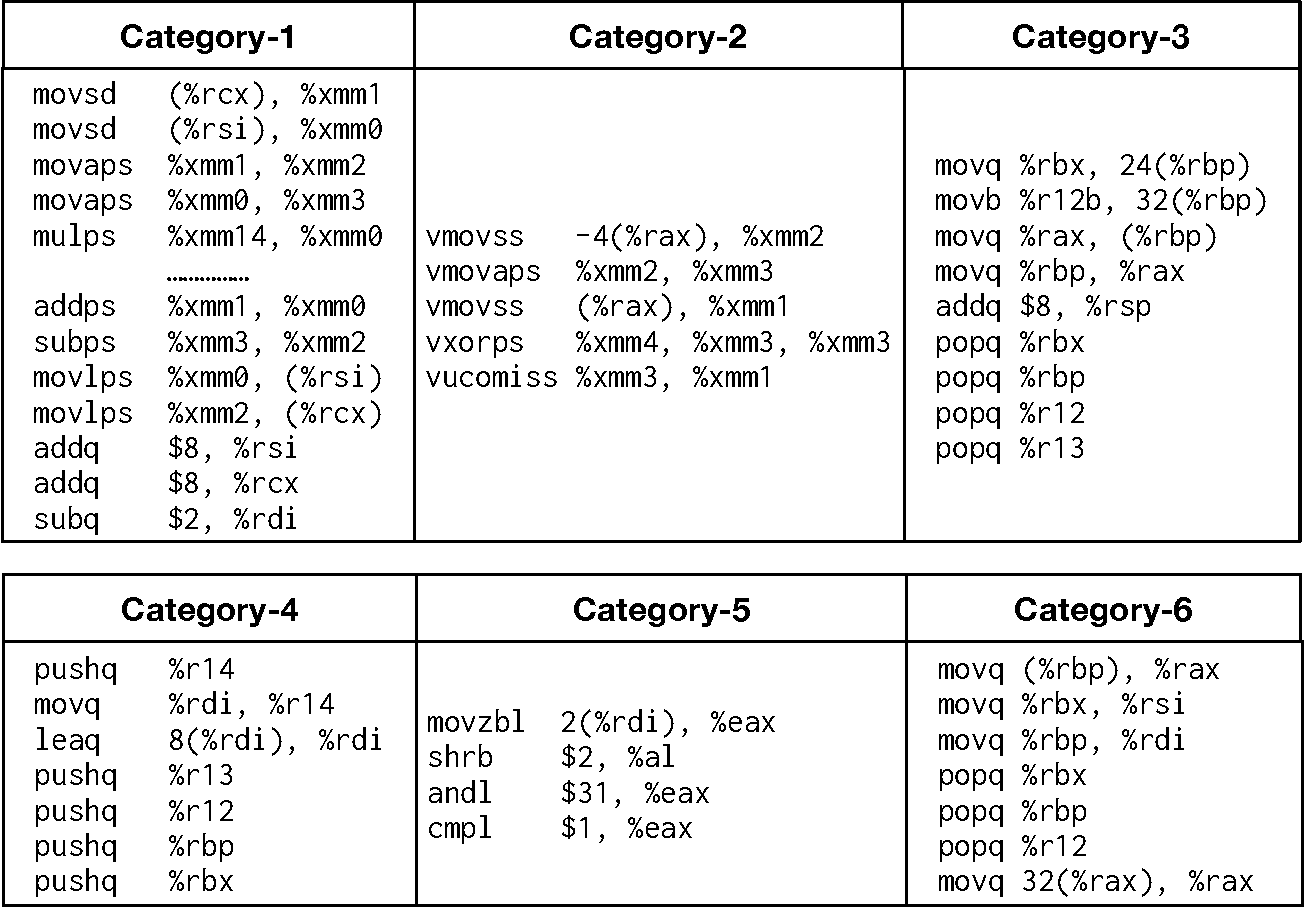
\includegraphics[width=\columnwidth]{figures/examples.pdf}
\caption{Example basic blocks for each category identified in Table~\ref{tab:categories}}
\label{fig:examples}
\end{center}
\end{figure}

% TODO: get a NICER figure
\begin{figure*}[h]
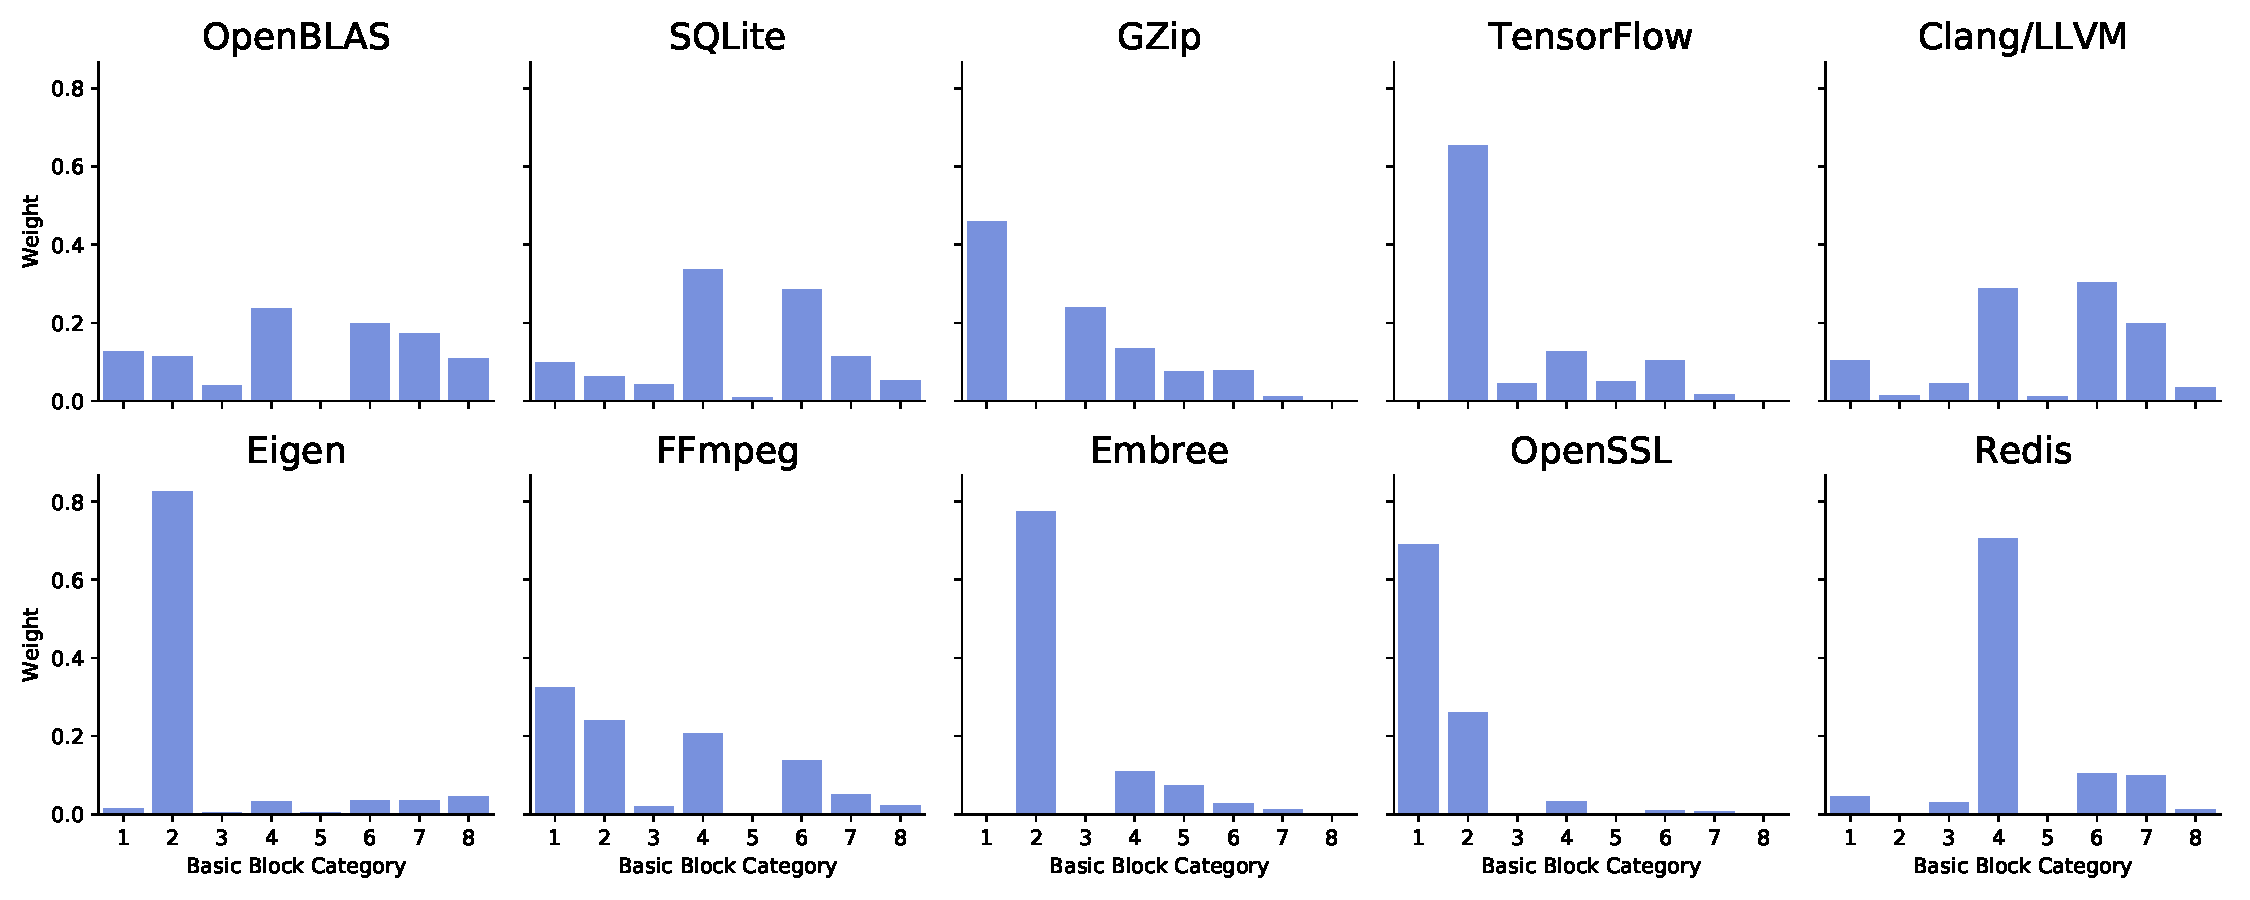
\includegraphics[width=\textwidth]{figures/apps-vs-clusters.pdf}
\caption{Breakdown of applications by basic block categories. The Y-axis is the percentage of basic blocks with the category specified on the X-axis. We define the category of a basic block as the most common category of micro-ops contained in the block.
Category-2 contains vectorized basic blocks.}
\label{fig:apps_vs_clusters}
\end{figure*}